\documentclass[10pt,letterpaper,subeqn]{beamer}
\setbeamertemplate{navigation symbols}{}
\usefonttheme{serif}
\usecolortheme{orchid}



\usepackage[english]{babel}
\selectlanguage{english}
\usepackage{amsmath, amsfonts, amssymb, cancel}
\usepackage{bm}
\usepackage{booktabs}
\usepackage{color}
\usepackage[update,prepend]{epstopdf}
\usepackage{framed}
\usepackage{fleqn}
\usepackage{graphics}
\usepackage{hyperref}
\usepackage[utf8]{inputenc}
\usepackage{setspace}
\usepackage{textcomp}
\usepackage{wrapfig}
\usepackage{multirow}
\usepackage{caption}
%\usepackage{subcaption}
\usepackage{lscape}
\setbeamertemplate{caption}[numbered]



\title{Assessing Plan B: The Effect of the Morning After Pill on Children and Women}
\author{Andrea Bentancor\inst{1} \and Damian Clarke\inst{2}}
\institute{\inst{1} Universidad Adolfo Ib\'a\~nez  \inst{2} University of Oxford}
\date{December 2014}


\begin{document}


\begin{frame}
\titlepage
\end{frame}

\section{This Talk}
%\frame{\frametitle{This Talk}
%\begin{enumerate}
%\item There was \textcolor{blue}{quasi-experimental} variation in fully-subsidised
%\textcolor{blue}{morning after pill} availability in Chile. \vspace{2mm}
%\item Availability \textcolor{blue}{reduced teenage childbearing} and (illegal) 
%abortions by an important amount. \vspace{2mm}
%\item The control group may be partially treated via \textcolor{blue}{spillovers}.  
%Show how to recover consistent estimates.
%\end{enumerate}
%}

\frame{\frametitle{This Talk (I)}
We make an empirical point.  Essentially:
\begin{figure}[htpb!]
\begin{center}
\caption{Trends in Pregnancy (15-19 year-olds) Chile}
\label{TEENfig:Reform}
\vspace{-6mm}
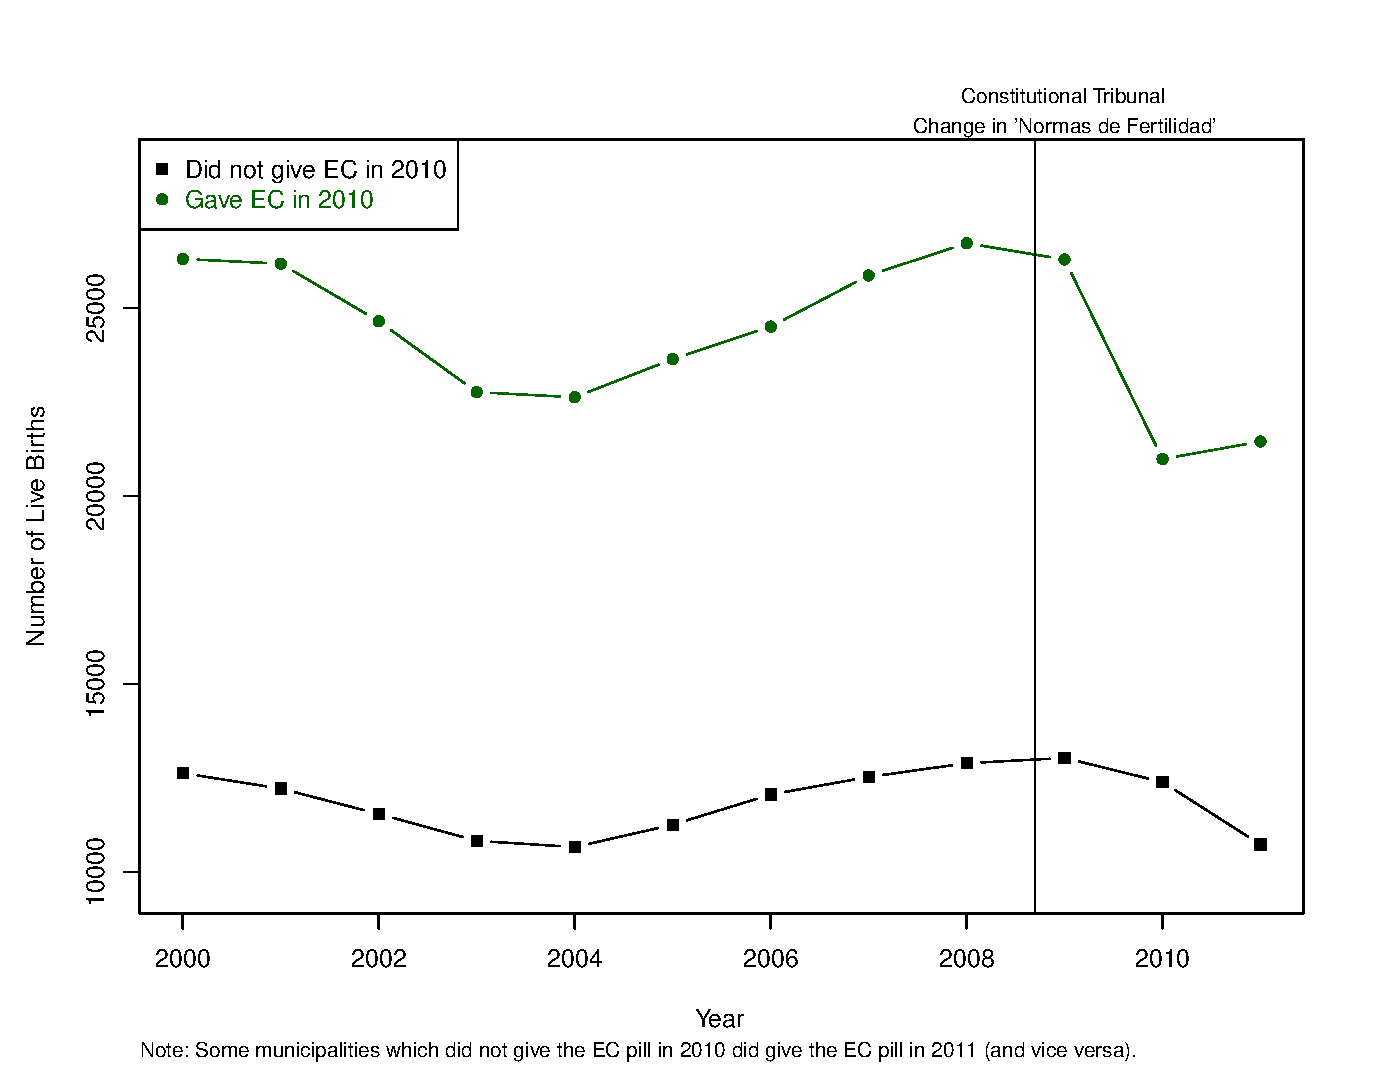
\includegraphics[scale=0.35]{./../../Figures/Reform1519.eps}
\end{center}
\end{figure}
}

\frame{\frametitle{This Talk (II)}
We also make a theoretical point:
\vspace{5mm}
\begin{itemize}
\item Estimation in differences-in-differences (DD) is frequently based on permeable 
boundaries (ie state, municipality)
\item SUTVA-type considerations are necessarily invoked, despite the chance of local spillovers
\item We show that SUTVA can be loosened in an empirical framework to flexibly identify:
\begin{enumerate}
\item The headline treatment effect
\item The effect of treatment spillover \emph{across} spatial boundaries
\end{enumerate}
\item We show that these types of spillovers are likely to result in attenuation bias in DD estimates
\end{itemize}
}


\section{Introduction}
\frame{
\begin{center}
\textcolor{blue}{{\Large\textsc{Introduction}}}
\end{center}
}

%\frame{\frametitle{Motivation}
%\begin{itemize}
%\item Considerable evidence that the oral contraceptive pill improves outcomes for women and children
%\begin{itemize}
%\item Delays in childbearing, marriage (Angrist and Evans, 1996)
%\item Higher education, labour market participation (Goldin and Katz, 2002)
%\item Reduction in gender wage differential (Bailey 2012)
%\end{itemize}
%\item But, \textcolor{blue}{scarce evidence on the effects of post-coital birth control}
%\item A small number of papers from expansions in USA, nothing outside USA, nor at national level
%\item Would like to know: how does the introduction of the ``morning after pill'' affect 
%fertility/abortions?
%\end{itemize}
%}

\frame{\frametitle{Importance}
\begin{itemize}
\item Oral contraceptive pill provided fundamental change in ability to control total fertility and timing (Bailey 2006)
\item However, requires a costly, ongoing and regular investment
\item The morning after pill however, is a once-off contraceptive (non-abortive) treatment
\item In many situations it is much cheaper or fully subsidised
\item Also, non-abortive, so present in circumstances even where abortion is illegal
\item May operate at a different margin (younger women and women not regularly contracepting)
\end{itemize}
}

\frame{\frametitle{Importance II}
Considerable polemic regarding the introduction of AE in Chile
\vspace{5mm}
\begin{itemize}
\item However, very little (or no?) evidence regarding \emph{effects} 
\item This in a context of high rates of adolescence pregnacy
\begin{itemize}
\item In Chile, \textcolor{red}{48.60 per 1000} women aged 15-19 (2012)
\item \emph{Very strong} correlation with poverty, vulnerability, education
\item Low rates of contraceptive coverage: \textcolor{red}{12.9\% of 15-19} year olds using any form (INJUV)
\end{itemize}
\item AE is likely to be particularly effective in Chile given the absence
of other post-coital birth control options
\end{itemize}
}

\frame{\frametitle{Importance III}
The `deep determinants' of teenage pregnancy include education, expectations and
outside opportunities (ie Wolfe et al 2001; Ripani et al 2014)
\vspace{5mm}
\begin{itemize}
\item However, \emph{even} where deep determinants are fulfilled, contraceptive 
technologies are a necessary condition to avoid undesired childbearing
\item Here we examine the effect of loosening a technological constraint (the 
absence of legal, safe post-coital contraceptive)
\item In the long run, theoretically at least, this leads to 
\textcolor{blue}{greater empowerment} in intra-household settings (Chiappori and Oreffice)
\end{itemize}
}

%\frame{\frametitle{Importance III}
%Econometrically, DD techniques require SUTVA, or the lack of a spillover between subjects
%\vspace{5mm}
%\begin{itemize}
%\item Literature recognises spillovers \emph{within} treatment clusters (Angelucci; Bobonis; Baird et al.)
%\item However, in this case we are concerned that plausibly exogenous treatment may cross \emph{beween} treatme%nt clusters
%\item If this is the case, control groups are partially contaminated
%\item We propose a flexible estimation technique to recover consistent estimates in the presence of local
%spillovers
%\end{itemize}
%}


\begin{frame}[label=Context]
\frametitle{The Context}
A finding by a Constitutional Tribunal in 2008 regarding \emph{las normas nacionales sobre la fertilidad} making the morning after pill legal, but at the discretion of each mayor in local jurisdictions (\emph{comunas})
\vspace{5mm}
\begin{itemize}
\item This is quite different to USA literature given that abortion is entirely outlawed in Chile
\item Previously, any person in Chile wanting to post coitally contracept had to:
\begin{itemize}
\item Risk illegal abortion which is prosecuted, dangerous and stigmatised; or
\item Have access to the information that high doses of the pill act similarly to the emergency contraceptive (EC) pill
\item Purchase the morning after pill (sporadically available from 1995)
\end{itemize}
\end{itemize}
\hyperlink{PAE}{\beamergotobutton{Further Details\ldots}}
\end{frame}

\frame{\frametitle{Roadmap: Findings}
\begin{itemize}
\item Na\"ive estimates of the reform suggest a \textcolor{blue}{4.0\%} and 3.0\% reduction in total pregnancies for 15-19 and 20-34 year olds respectively
\item Similarly, we find suggesting evidence that the morning after pill reduced abortions 
\item Once accounting for spillovers, main effects are a \textcolor{blue}{6.9\%} reduction in births (15-19) and a reduction of approximately 55\% in illegal abortion
\item These effects are not focused by a woman's labour market or educational status
\end{itemize}
}

\section{Methodology}
\frame{
\begin{center}
\textcolor{blue}{{\Large\textsc{Methodology}}}
\end{center}
}

\frame{\frametitle{Methodology}
\[
 \label{TEENeqn:pill}
birth_{ijt} = \alpha + \delta\cdot \mathbb{I}\{Pill_{jt-1}\} + \phi_t + \eta_j + 
\eta_j\cdot t + X_{jt-1}\gamma + \varepsilon_{ijt}.
\]
\vspace{5mm}
\begin{itemize}
\item Flexible diff-in-diffs
\item Woman $i$ in municipality $j$ and time $t$ is `treated' if public health
centres report that the pill is freely available upon request
\item Identifying assumption is parallel trends
\end{itemize}
}

\frame{\frametitle{Estimating Treatment Effects in The Presence of Treatment Spillovers}
\[
y_{ijct} = \alpha + \delta\cdot \mathbb{I}\{Pill_{jt-1}\} + 
\sum_{c=0}^C\zeta_c\cdot close_{cdjt-1} + \hdots + \varepsilon_{ijct}
\]
where
\[
 close_{cdjt} =
  \begin{cases}
   1 & \text{if } dist_{jt} > c \wedge dist_{jt}\leq c+d   \\
   0 & \text{if } dist_{jt} \leq c \vee  dist_{jt}>c+d.
  \end{cases}
\]
\vspace{5mm}
\begin{itemize}
\item Test what happens if we exclude from the control group women `close to' the pill
\item Let the data determine who is `close' and who isn't
\item This loosens SUTVA, but still requires that this hold in non-close municipalities
\item Cluster errors to allow for spatial correlation (Conley, 1999)
\end{itemize}
}


\begin{frame}[label=demo1]
\frametitle{Estimating Treatment Effects in The Presence of Treatment Spillovers}
In other words, we can include a series of dummies: $close_{0,10}$, $close_{10,20}$, 
$close_{20,30}$, \ldots
\vspace{5mm}
\begin{itemize}
\item We can include marginal `close' variables until either:
\begin{itemize}
\item The effect on the marginal close dummy (ie $close_{20,30}$) is identical to the effect 
on the dummy before (ie $close_{10,20}$)
\item Or the main effect $\hat{\delta}$ no longer varies as additional dummies are added
\end{itemize}
\item Thus, the only discretionary choice is the distance covered by each close dummy
\item \hyperlink{demonstrate}{\beamergotobutton{It can be shown}} that if spillovers work in 
the same direction as treatment (ie reduce births),
then omitting close dummies biases $\hat\delta$ towards zero
\end{itemize}
\end{frame}


\frame{\frametitle{General Identification Challenges}
Parallel trends assumption would be violated if pill and non-pill mayors simultaneously embark
on other related policies
\begin{itemize}
\item Selection into prescribing the pill is largely based on mayor's ideology, however not
necessarily along party lines
\item Pill law was passed mid-electoral cycle
\item Add a series of time-varying controls
\begin{itemize}
\item Fundamentally, this includes other contraceptive dispursement (condoms) and education and health spending
\end{itemize}
\item Undertake a series of robustness checks using false (lagged) treatments
\end{itemize}
}

\section{Data}
\frame{
\begin{center}
\textcolor{blue}{{\Large\textsc{Data}}}
\end{center}
}


\frame{\frametitle{The Reform}
Constitutional finding of the Supreme Court in 2008 regarding ``National Laws for the Regulation
of Fertility'' (Law 20.418)
\begin{itemize}
\item Made it legal for all Municipal Health Centres to distribute the EC pill freely to women
\item Of the 346 municipalities in Chile, approximately 150 immediately reported that they 
distribute the EC pill without restriction
\item EC pill prescriptions jumped sharply, from 0 in 2007 to approximately 7,000 doses in 2008
\end{itemize}
}

\frame{
\begin{figure}[htpb!]
\begin{center}
\caption{Pill Prescriptions and Availability by Time}
\label{TEENfig:Pilltime}
\vspace{-5mm}
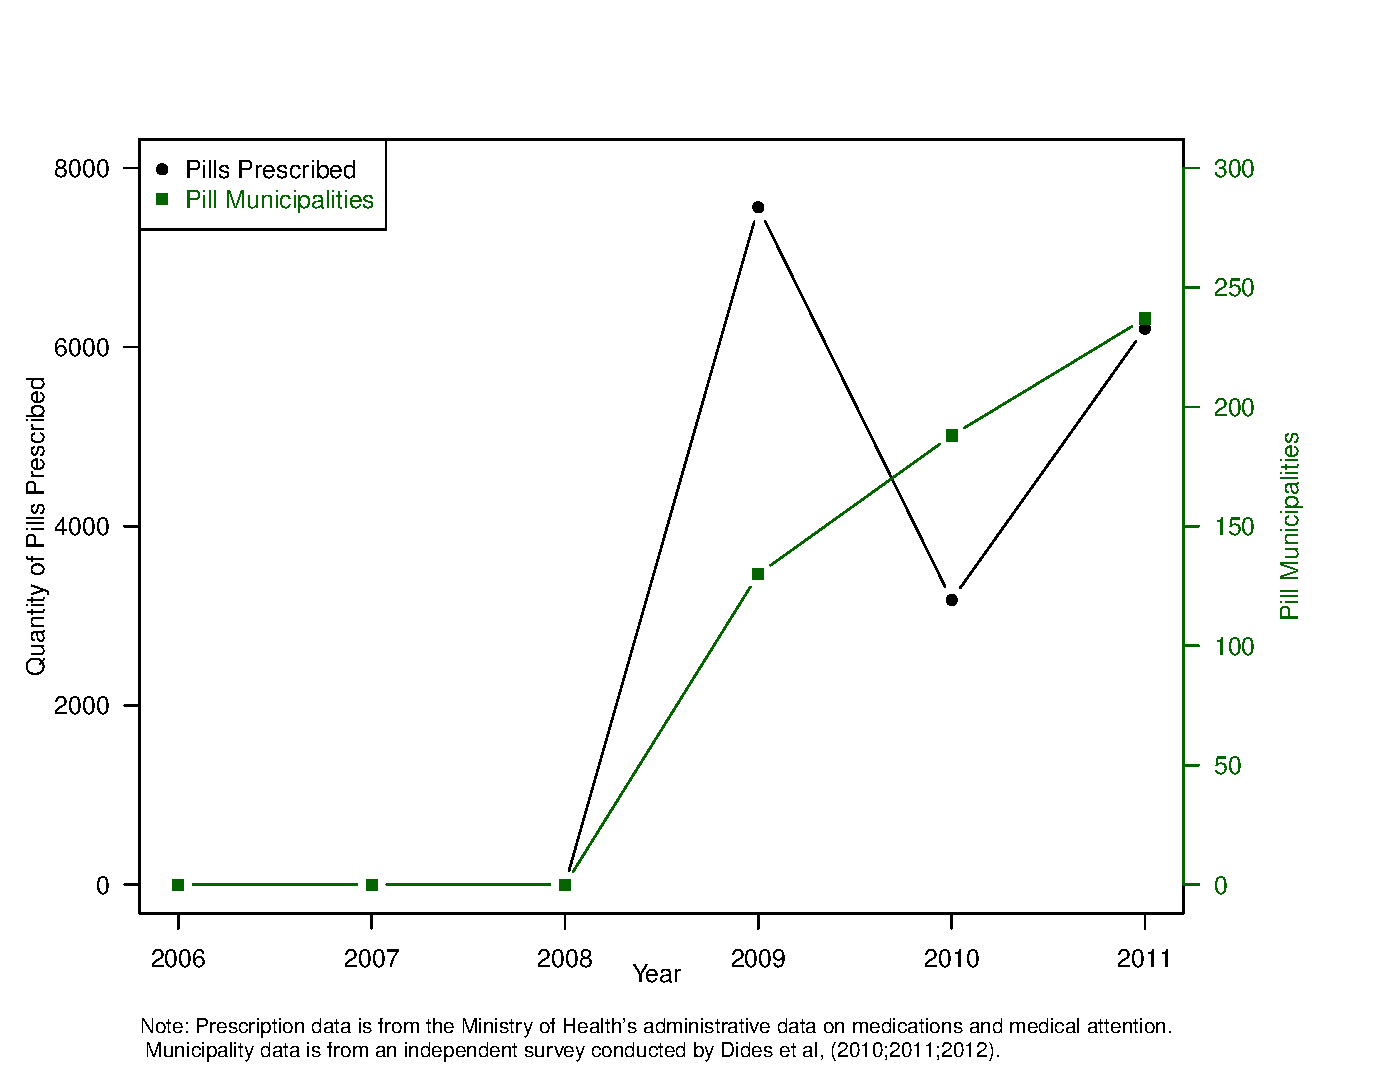
\includegraphics[scale=0.44]{./../../Figures/Pill.eps} 
\end{center}
\end{figure}
}

\frame{
\begin{figure}[htpb!]
\begin{center}
\caption{The Availability of the Pill by Geographic Region}
\label{TEENfig:PillGeo}
\includegraphics[scale=0.2]{./../../Results/Pill/Pill_l.eps}
\end{center}
\end{figure}
}

\begin{frame}[label=sum]
\frametitle{Data}
\begin{itemize}
\item Matched administrative data files recording all live births and fetal deaths in Chile
\item Crossed with data recording population by municipality.  Principal outcomes:
\begin{itemize}
\item Births per woman
\item Fetal deaths per live birth (late term, early term)
\end{itemize}
\item All births and deaths from 2006--2011.  1,391,565 births; 11,387 fetal deaths
\item Measure of treatment comes from an independent survey (Dides et al.\ 2009, 2010, 2011)
\item Also have administrative data on pill disbursements
\end{itemize}
\hyperlink{sumR}{\beamergotobutton{Descriptives}}
\end{frame}




\frame{
\begin{figure}[htpb!]
\begin{center}
\caption{Total Recorded Births and Fetal Deaths, 2006-2011}
\label{TEENfig:BirthDeath}
\vspace{-5mm}
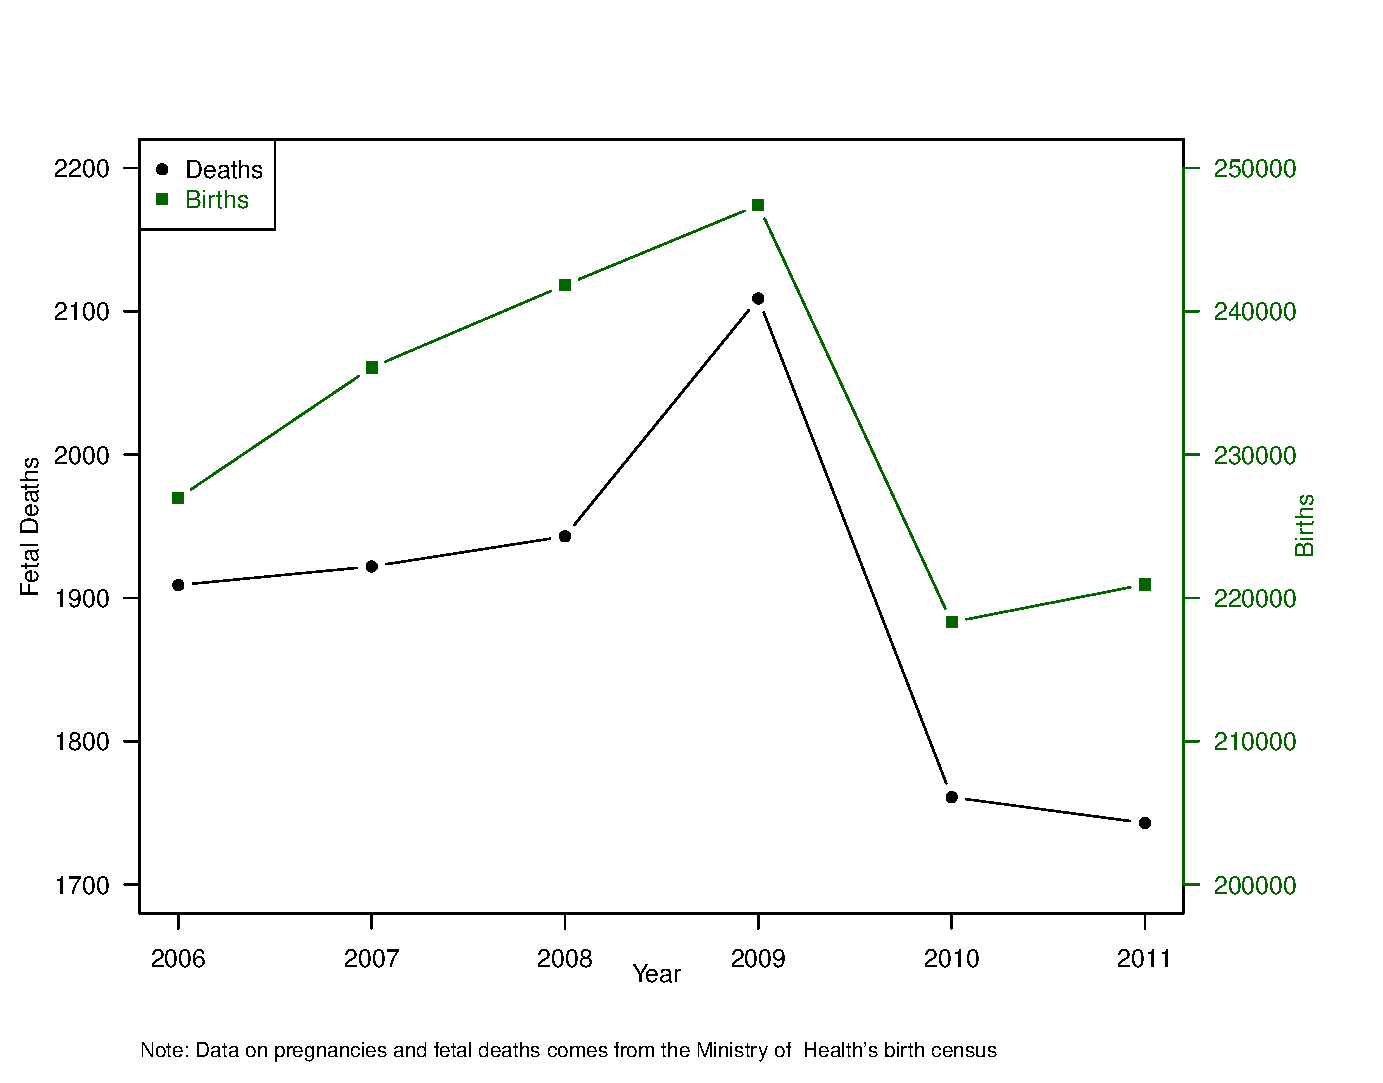
\includegraphics[scale=0.44]{./../../Figures/BirthDeath.eps} 
\end{center}
\end{figure}
}

\section{Results}
\frame{
\begin{center}
\textcolor{blue}{{\Large\textsc{Results}}}
\end{center}
}

\frame{\frametitle{Results}
Headline results:
\begin{itemize}
\item Na\"ive estimates of the effect of having the morning after pill available:
\begin{itemize}
\item Reduces births by 4.0\% for teenagers
\item Reduces births by 3.0\% for 20-34 year olds
\item No effect on 35-44 year olds
\item Strong evidence for reduction in early term fetal deaths, no effect on late term
\end{itemize}
\item However, strong evidence of spillovers.  Those living `close to' pill municipalities 
also have:
\begin{itemize}
\item Reduction in births for 15--19, 20--34 year olds
\item Reduced rates of early-term fetal deaths
\item These effects persist for distances up to 30km\ldots
\end{itemize}
\end{itemize}
}

\frame{\frametitle{Births}
\begin{landscape}
\begin{table}[!htbp] \centering
\caption{The Effect of the Morning After Pill on Pregnancy}
\vspace{-6mm}
\label{TEENtab:PillPreg}
\scalebox{0.46}{
\begin{tabular}{@{\extracolsep{5pt}}lccccp{1mm}cccc}
\\[-1.8ex]\hline \hline \\[-1.8ex] 
&\multicolumn{4}{c}{All Births}&&\multicolumn{4}{c}{First Births}
\\ \cmidrule(r){2-5} \cmidrule(r){7-10}
&(1)&(2)&(3)&(4)&&(5)&(6)&(7)&(8)\\ \hline
\multicolumn{10}{l}{\textsc{\noindent 15-19 year olds}} \\
 & & & & & & & & & \\
Morning After Pill &$-$0.064$^{***}$&$-$0.065$^{***}$&$-$0.057$^{***}$&$-$0.041$^{***}$&&$-$0.036$^{**}$&$-$0.041$^{***}$&$-$0.036$^{**}$&$-$0.021\\
 &(0.013)&(0.014)&(0.014)&(0.014)&&(0.014)&(0.015)&(0.015)&(0.015)\\
 & & & & & & & & & \\
Observations&4,152,490&4,152,490&4,152,490&4,152,490&&4,125,336&4,125,336&4,125,336&4,125,336\\
McFadden's $R^2$&0.670&0.670&0.671&0.673&&0.633&0.634&0.636&0.637\\
 & & & & & & & & & \\
\multicolumn{10}{l}{\textsc{\noindent 20-34 year olds}} \\
 & & & & & & & & & \\
Morning After Pill &$-$0.040$^{***}$&$-$0.039$^{***}$&$-$0.038$^{***}$&$-$0.030$^{***}$&&$-$0.024$^{*}$&$-$0.029$^{**}$&$-$0.029$^{**}$&$-$0.021\\
 &(0.010)&(0.010)&(0.010)&(0.010)&&(0.012)&(0.013)&(0.014)&(0.014)\\
 & & & & & & & & & \\
Observations&11,022,111&11,022,111&11,022,111&11,022,111&&10,458,703&10,458,703&10,458,703&10,458,703\\
McFadden's $R^2$&0.772&0.772&0.773&0.774&&0.684&0.685&0.686&0.686\\
 & & & & & & & & & \\
\multicolumn{10}{l}{\textsc{\noindent 35-49 year olds}} \\
 & & & & & & & & & \\
Morning After Pill &0.001&0.001&0.008&0.006&&0.042&0.039&0.042&0.033\\
 &(0.012)&(0.012)&(0.012)&(0.012)&&(0.033)&(0.034)&(0.034)&(0.035)\\
 & & & & & & & & & \\
Observations&10,572,196&10,572,196&10,572,196&10,572,196&&10,376,895&10,376,895&10,376,895&10,376,895\\
McFadden's $R^2$&0.537&0.537&0.538&0.538&&0.641&0.641&0.642&0.642\\
\hline \\[-1.8ex] 
{\small Trends \& FEs} & Y & Y & Y & Y && Y & Y & Y & Y \\
{\small Political Controls} & & Y & Y & Y && & Y & Y & Y \\
{\small Health, Educ, Gender Controls} & & & Y & Y && & & Y & Y \\
{\small Condom Availability} & & & & Y && & & & Y \\
\hline \hline \\[-1.8ex]
\multicolumn{10}{p{22cm}}{\begin{footnotesize}\textsc{Notes:}
$^{*}$p$<$0.1; $^{**}$p$<$0.05; $^{***}$p$<$0.01\end{footnotesize}}
\normalsize\end{tabular}}\end{table}\end{landscape}

}

\frame{\frametitle{Fetal Deaths}
\begin{table}[htpb!] \centering
\caption{The Effect of the Morning After Pill on Fetal Deaths}
\vspace{-2mm}
\label{TEENtab:PillDeath}
\scalebox{0.54}{
\begin{tabular}{@{\extracolsep{5pt}}lccc}\\[-1.8ex]
\hline\hline\\[-1.8ex]
& All & Early & Late \\
& Deaths & Gestation & Gestation \\ \midrule
\multicolumn{4}{l}{\textsc{15-19 year olds}} \\
&&&\\
Morning After Pill &$-$0.131&$-$0.728$^{***}$&$-$0.078\\
&(0.083)&(0.189)&(0.113)\\
&&&\\
Mean (deaths/live birth)&0.008&0.002&0.005\\
Observations&219,608&218,388&218,911\\
McFadden's $R^2$&0.233&0.379&0.254\\
&&&\\
\multicolumn{4}{l}{\textsc{20-34 year olds}} \\
&&&\\
Morning After Pill &$-$0.041&$-$0.139&$-$0.035\\
&(0.049)&(0.106)&(0.057)\\
&&&\\
Mean (deaths/live birth)&0.007&0.002&0.004\\
Observations&954,424&949,477&951,577\\
McFadden's $R^2$&0.199&0.386&0.171\\
&&&\\
\multicolumn{4}{l}{\textsc{35-49 year olds}} \\
&&&\\
Morning After Pill &$-$0.460$^{***}$&$-$0.738$^{***}$&$-$0.502$^{***}$\\
&(0.081)&(0.216)&(0.101)\\
&&&\\
Mean (deaths/live birth)&0.012&0.003&0.007\\
Observations&228,920&227,029&227,781\\
McFadden's $R^2$&0.261&0.411&0.239\\
\hline \hline \\[-1.8ex]
\multicolumn{4}{p{10cm}}{\begin{footnotesize}\textsc{Notes:}
$^{*}$p$<$0.1; $^{**}$p$<$0.05; $^{***}$p$<$0.01;\end{footnotesize}}
\normalsize\end{tabular}}\end{table}

}

\frame{\frametitle{Spillovers}
\begin{table}[!htbp] \centering
\caption{The Morning After Pill and Treatment Spillovers}
\label{TEENtab:Spillover} 
\scalebox{0.5}{\begin{tabular}
{@{\extracolsep{5pt}}lccc}\\[-1.8ex]\hline\hline\\
[-1.8ex] & 15-19 & 20-34 & 35-49 \\
& Year olds & Year olds & Year olds \\ \midrule
\multicolumn{4}{l}{\textsc{\noindent Panel A: Births}} \\
& & & \\
Morning After Pill &$-$0.091$^{***}$&$-$0.053$^{***}$&0.016\\
&(0.016)&(0.013)&(0.014)\\
Close $<15$ km &$-$0.083$^{***}$&$-$0.044$^{***}$&0.019\\
&(0.021)&(0.014)&(0.016)\\
Close 15-30 km &$-$0.078$^{***}$&$-$0.024$^{*}$& \\
&(0.022)&(0.013)& \\
Close 30-45 km &$-$0.057&$-$0.026& \\
&(0.036)&(0.031)& \\
& & & \\
Observations&4,152,490&11,022,111&10,572,196\\
McFadden's $R^2$&0.673&0.774&0.538\\ \midrule
\multicolumn{4}{l}{\textsc{\noindent Panel B: Fetal Deaths}}\\
&&&\\
Morning After Pill &$-$0.935$^{***}$&$-$0.230$^{*}$&$-$0.785$^{***}$\\
&(0.217)&(0.125)&(0.230)\\
Close $<15$ km &$-$0.163&$-$0.031& 0.051\\
&(0.234)&(0.151)&(0.226)\\
&&&\\
Observations&218,388&949,477&227,029\\
McFadden's $R^2$&0.379&0.386&0.412\\
\hline \hline \\[-1.8ex]
\end{tabular}}\end{table}

}

\begin{frame}[label=dist1519]
\begin{figure}[htpb!]
\begin{center}
\caption{Estimates of $\hat\delta^c$ for Pregnancy (15-19)}
\label{TEENfig:Dist1519}
\vspace{-5mm}
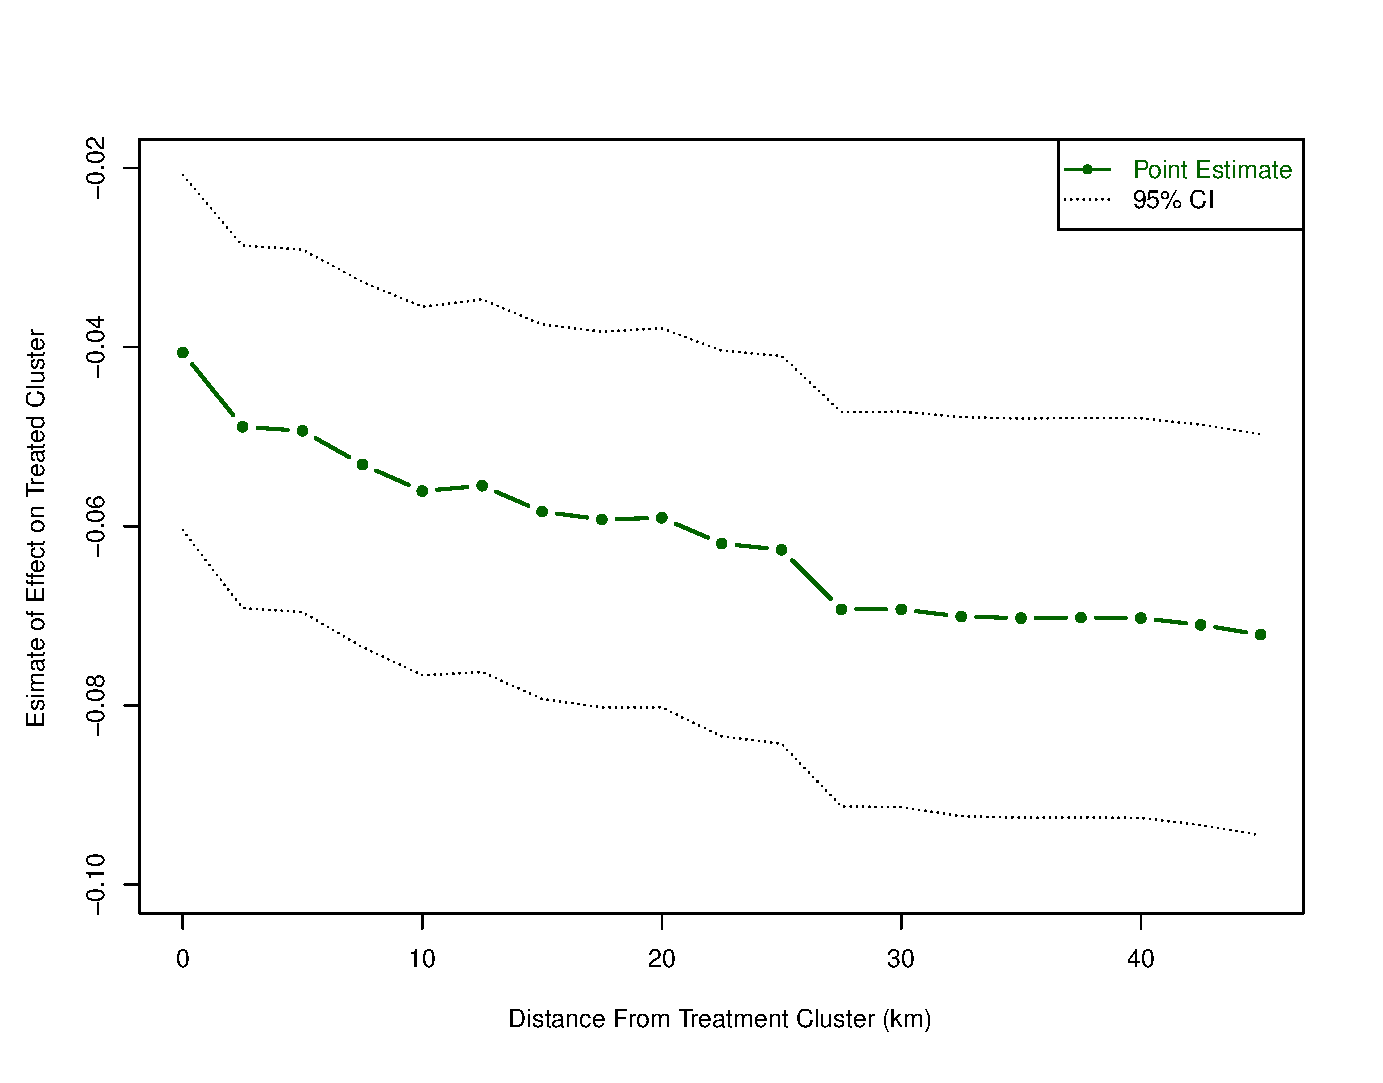
\includegraphics[scale=0.44]{./../../Figures/Dist1519.eps} 
\end{center}
\end{figure}
\hyperlink{dist2034}{\beamergotobutton{20-34 year-olds}}
\end{frame}

\begin{frame}[label=plaus]
\frametitle{Plausibility?}
These are large effects, and indeed much larger than what is reported in the two economic studies that exist in the USA.  However:
\begin{itemize}
\item These effects are similar in magnitude to the effect of viewing ``16 and Pregnant'' (Kearney and Levine, 2014)
\item In Chile, prior to the morning after pill, outside options were very limited: either give birth, travel to abort, or risk death/incarceration in the country
\item In cases where abortion exists, this technology may shift women from abortion to post-coital contraceptives, and so may not turn up in net figures
\item A back of the envelope calculation suggests that the effectiveness of the pill (pregnancies avoided per prescription) is $\sim$0.7-0.8.  The US FDA suggests that typical use has effectiveness of 89\%
\hyperlink{plausR}{\beamergotobutton{See results}}
\end{itemize}
\end{frame}

\frame{\frametitle{Placebo Tests}
We can run similar regressions comparing pill and non-pill $comunas$ using false (lagged) reforms:
\begin{equation}
 \label{TEENeqn:placebo}
\nonumber
birth_{ijt-l} = \alpha + \delta\cdot \mathbb{I}\{Pill_{jt}\} + \phi_t + \eta_j + 
\eta_j\cdot t + \varepsilon_{ijt},
\end{equation}
\vspace{5mm}
\begin{itemize}
\item Where $l$ refers to a series of lags $l\in 3,4,5$ years.
\item We should expect that in each case, $\hat\delta$ should not be significantly different to zero 
\end{itemize}
}

\frame{\frametitle{Placebo Tests}
\begin{landscape}
\begin{table}[!htbp] \centering
\caption{Placebo Tests}
\vspace{-7mm}
\label{TEENtab:Placebo}
\scalebox{0.56}{
\begin{tabular}{lcccccc}
\\[-1.8ex]\hline \hline \\[-1.8ex] 
&\multicolumn{2}{c}{Lag = 3 years}
&\multicolumn{2}{c}{Lag = 4 years}
&\multicolumn{2}{c}{Lag = 5 years}
\\ \cmidrule(r){2-3} \cmidrule(r){4-5} \cmidrule(r){6-7}
&(1)&(2)&(3)&(4)&(5)&(6)\\ \hline
\textsc{Panel A: 15-19 Year-Olds} &&&&&& \\
 & & & & & & \\
Morning After Pill &0.006&$-$0.018&0.003&$-$0.004&0.006&$-$0.018\\
&(0.014)&(0.017)&(0.014)&(0.029)&(0.014)&(0.017)\\
Close $<15$ km &&$-$0.047$^{**}$&& 0.021&&0.049\\
&&(0.022)&&(0.036)&&(0.041)\\
Close 15-30 km &&$-$0.001&&$-$0.046&&0.038\\
&&(0.022)&&(0.034)&&(0.040)\\
Close 30-45 km &&$-$0.047$^{*}$&&$-$0.028&&0.089$^{**}$\\
&&(0.025)&&(0.035)&&(0.041)\\
 & & & & & & \\
Observations&4,123,049&4,123,049&4,075,854&4,075,854&4,017,339&4,017,339\\
McFadden's $R^2$&0.235&0.235&0.235&0.235&0.239&0.239\\ \midrule
\textsc{Panel A: 20-34 Year-Olds} &&&&&& \\
 & & & & & & \\
Morning After Pill &0.000& 0.002&$-$0.006& 0.006&0.000& 0.002\\
&(0.008)&(0.017)&(0.008)&(0.019)&(0.008)&(0.017)\\
Close $<15$ km && 0.008&& 0.027&&$-$0.010\\
&&(0.017)&&(0.022)&&(0.021)\\
Close 15-30 km &&$-$0.005&& 0.002&& 0.009\\
&&(0.018)&&(0.021)&&(0.019)\\
Close 30-45 km &&$-$0.001&&$-$0.004&& 0.030\\
&&(0.019)&&(0.024)&&(0.020)\\
 & & & & & & \\
Observations&10,773,289&10,773,289&10,699,388&10,699,388&10,639,773&10,639,773\\
McFadden's $R^2$&0.232&0.232&0.221&0.221&0.219&0.219\\  \hline \hline
\multicolumn{7}{p{17.2cm}}{\begin{footnotesize}\textsc{Notes:}
$^{*}$p$<$0.1; $^{**}$p$<$0.05; $^{***}$p$<$0.01.\end{footnotesize}}
\normalsize\end{tabular}}\end{table}\end{landscape}

}

\frame{
\begin{figure}
\begin{center}
\caption{Birth Trends 2000-2011: 15-19 Years}
\vspace{-5mm}
\label{TEENfig:Trend2034}
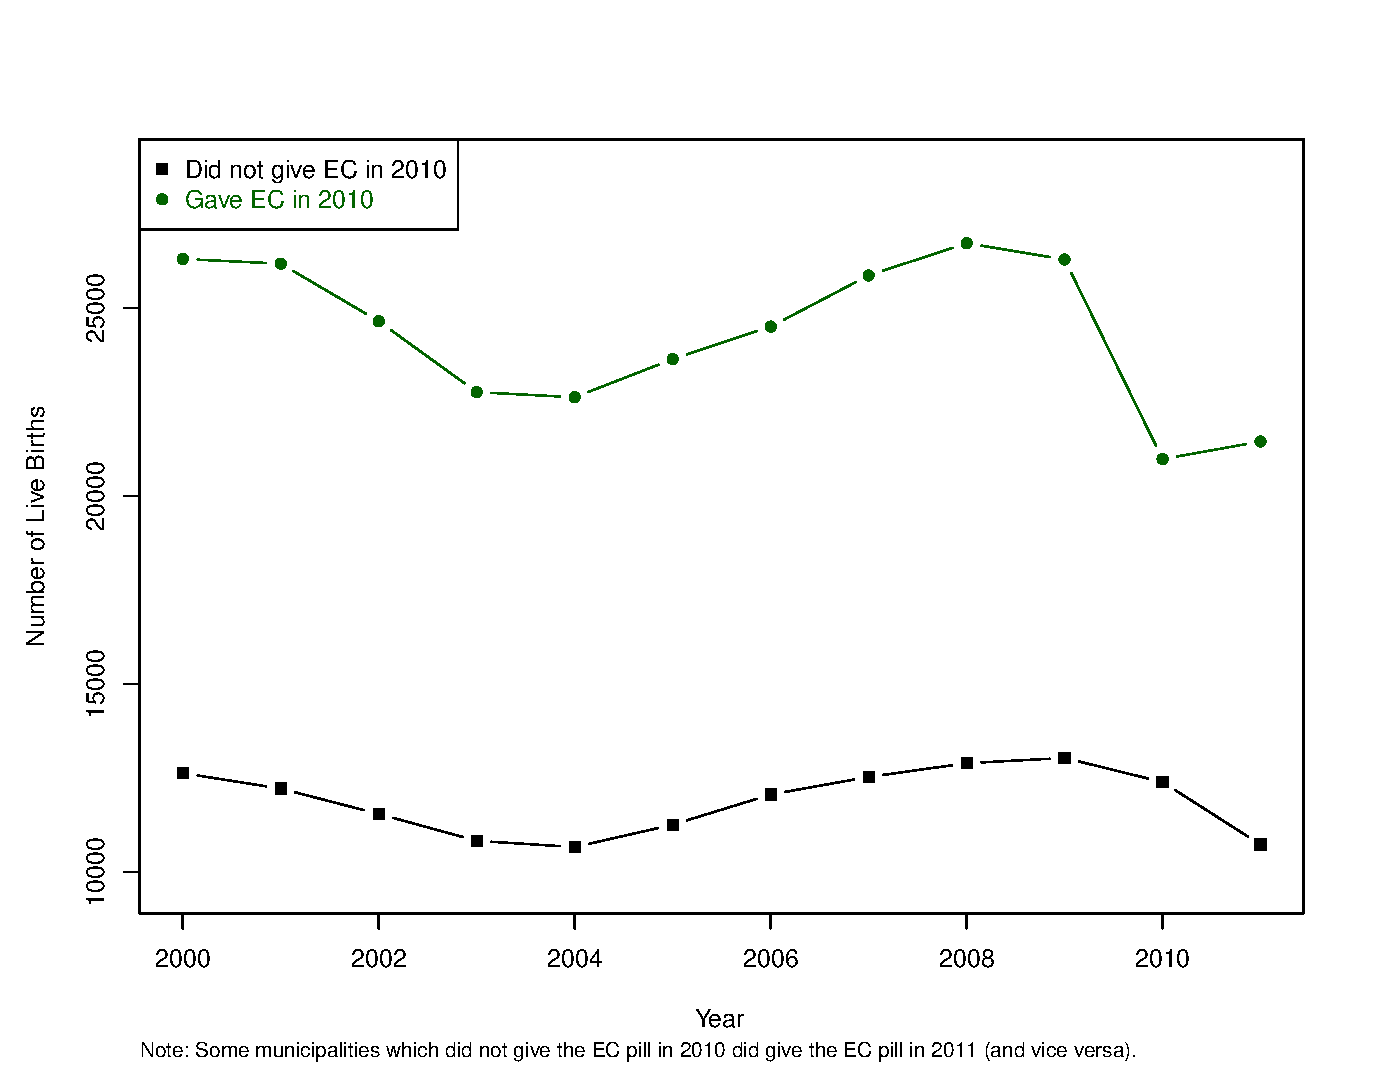
\includegraphics[scale=0.44]{./../../Figures/Trends1519.eps} 
\end{center}
\end{figure}
}


\frame{
\begin{figure}
\begin{center}
\caption{Birth Trends 2000-2011: 20-34 Years}
\vspace{-5mm}
\label{TEENfig:Trend2034}
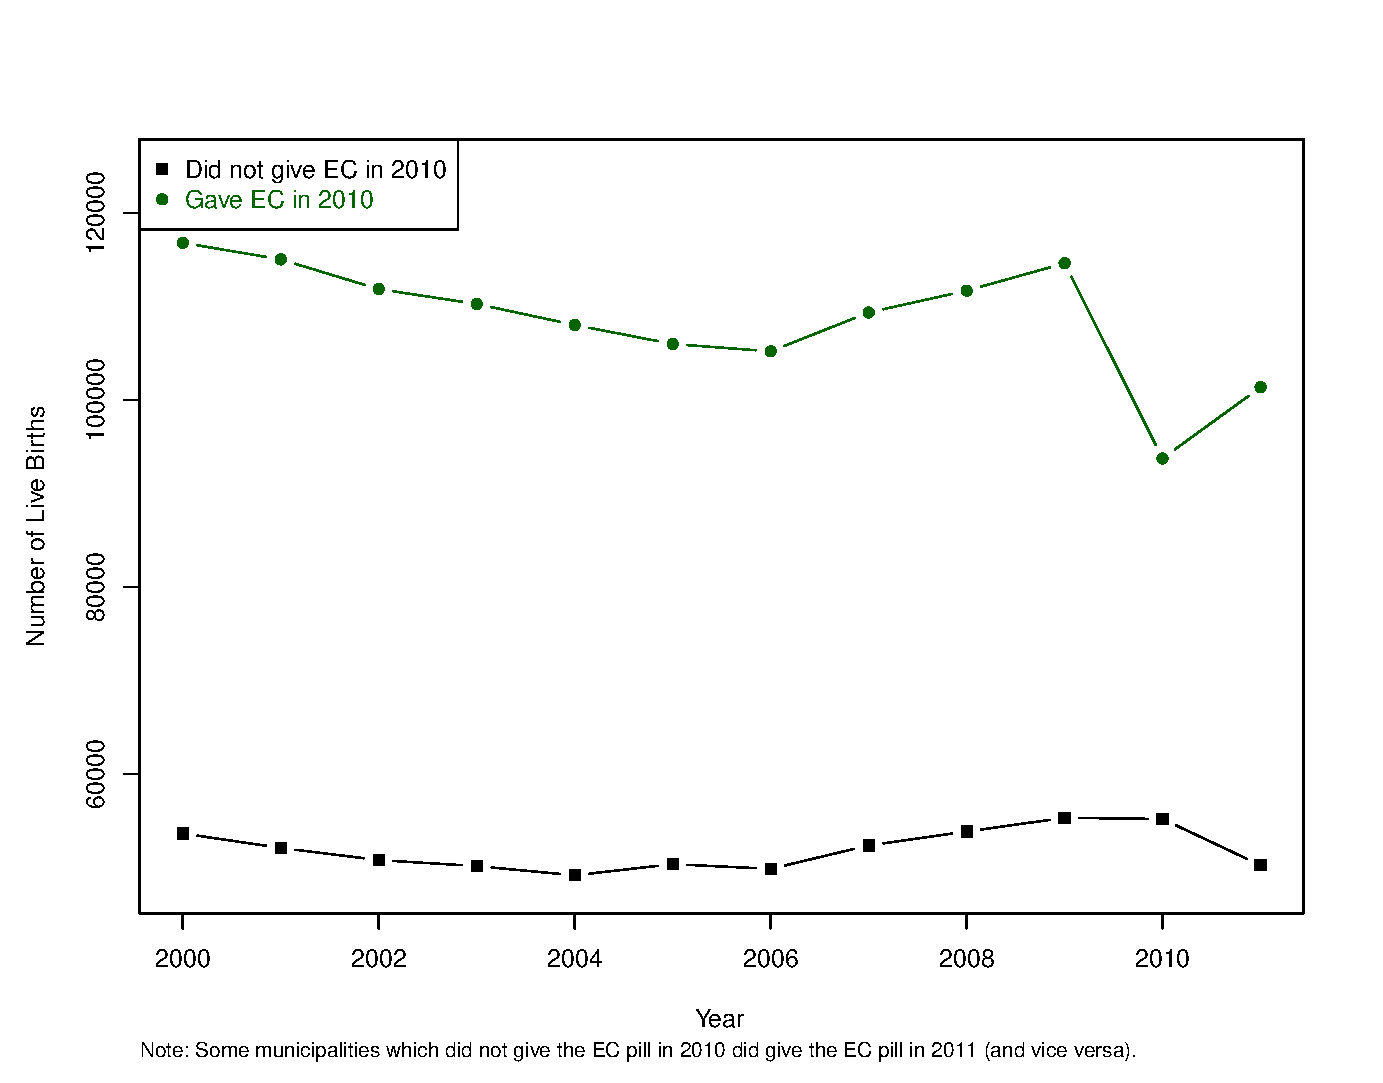
\includegraphics[scale=0.44]{./../../Figures/Trends2034.eps} 
\end{center}
\end{figure}
}


\section{Conclusion}
\frame{
\begin{center}
\textcolor{blue}{{\Large\textsc{Conclusion}}}
\end{center}
}

\frame{\frametitle{The Take Away Points}
\begin{enumerate}
\item There was \textcolor{blue}{quasi-experimental} variation in fully-subsidised
\textcolor{blue}{morning after pill} availability in Chile. \vspace{2mm}
\item Availability \textcolor{blue}{reduced teenage childbearing} and (illegal) 
abortions by an important amount. \vspace{2mm}
\item The control group may be partially contaminated via \textcolor{blue}{spillovers}.  
Show how to recover consistent estimates.
\end{enumerate}
\vspace{8mm}
All code is available on the web: \texttt{github.com/damiancclarke/morning-after-pill}
}

\frame{
\textcolor{blue}{Thank you.}
}

\section{Appended Details}
\frame{
\begin{center}
\textcolor{blue}{{\Large\textsc{Appended Details}}}
\end{center}
}

\begin{frame}[label=PAE]
\frametitle{The Morning After Pill in Chile}
In Chile, levonorgestrel is prescribed as a post-coital contraceptive to prevent the implantation
of the blastocyst\\
\vspace{5mm}
\begin{itemize}
\item The legislative environment surrounding this medication is complex (Casas-Becerra; Dides)
\begin{itemize}
\item ICMER began discussions in 1996
\item First sale was of Postinor in 2001 (resolution by Institute of Public Health)
\item Constitutionality was quickly challenged by NG groups; prohibited by Supreme Court
\item In November 2005 vote of Supreme Court votes 5-0 to reverse 2011 decision
\item 36 \emph{diputados} challenged this decision, going to Consititutional Tribunal
\end{itemize}
\item This paper begins in 2008, where Municipalities were allowed to prescribe
\end{itemize}
\hyperlink{Context}{\beamergotobutton{Back}}
\end{frame}

\begin{frame}[label=sumR]
\begin{table}[htpb!] \centering
\caption{Summary Statistics} \label{TEENtab:SumStats}
\begin{tabular} {@{\extracolsep{5pt}}lp{3mm}ccc}\\ [-1.8ex]
\hline\hline\\ [-1.8ex] &&No Pill&Pill&Total \\
&&Available&Available& \\ \midrule 
\multicolumn{5}{l}{\textbf{Municipality Characteristics}} \\
&&&& \\
Poverty &&16.4&17.0&16.6\\
&&(7.47)&(7.56)&(7.49) \\
Conservative &&0.286&0.267&0.281\\
&&(0.452)&(0.443)&(0.45) \\
Education Spending (Total) &&4,817&5,980&5,108\\
&&(5,649)&(6,216)&(5,818) \\
Education Spending (Municipal) &&430,625&525,143&454,232\\
&&(873,448)&(858,240)&(870,635) \\
Health Spending &&1,866&2,788&2,096\\
&&(2,635)&(3,381)&(2,867) \\
Out of School &&4.07&3.98&4.05\\
&&(3.16)&(3.06)&(3.13) \\
Female Mayor &&0.120&0.134&0.123\\
&&(0.325)&(0.341)&(0.329) \\
Female Poverty &&60.5&62.0&60.8\\
&&(10.64)&(9.48)&(10.4) \\
Condom Use &&0.466&0.536&0.483\\
&&(0.0506)&(0.0401)&(0.0571) \\
Pill Distance &&204&0.00&153\\
&&(5,229)&(0.00)&(4,530) \\
\multicolumn{5}{l}{\textbf{Individual Characteristics}}\\
&&&& \\
Live Births &&0.054&0.053&0.054\\
&&(0.226)&(0.224)&(0.226) \\
Fetal Deaths &&0.0558&0.0513&0.0547\\
&&(0.269)&(0.256)&(0.266) \\
Birthweight &&3322.7&3334.3&3324.7\\
&&     (540.0)&     (542.3)&     (540.4)\\
Maternal education  &&       11.92&       12.03&       11.94\\
&&     (2.967)&     (2.894)&     (2.955)\\
Percent working     &&       0.295&       0.395&       0.312\\
&&     (0.456)&     (0.489)&     (0.463)\\
Married     &&       0.340&       0.309&       0.335\\
&&     (0.474)&     (0.462)&     (0.472)\\
Age at Birth      &&       27.05&       27.15&       27.07\\
&&     (6.777)&     (6.790)&     (6.779)\\ \midrule
N Comunas &&336&280&336\\
N Fetal Deaths &&9,999&3,064&13,063\\
N Births &&1,214,088&391,212&1,605,300\\
\hline \hline \\[-1.8ex]
\multicolumn{5}{p{12cm}}{\begin{footnotesize}\textsc{Notes:}
Group means are presented with standard deviations below in
parentheses.  Poverty refers to the \% of the municipality
below the poverty line, conservative is a binary variable
indicating if the mayor comes from a politically conservative
party (UDI or RN), health and education spending are measured
 in thousands of Chilean
pesos, and pill distance measures the distance (in km) to the
nearest municipality which reports prescribing emergency
contraceptives.  Pregnancies are reported as \% of all women
giving live birth, while fetal deaths are reported per live
birth.  All summary statistics are for the period 2006-2012.
\end{footnotesize}} \normalsize\end{tabular}\end{table}

\hyperlink{sum}{\beamergotobutton{Back}}
\end{frame}

\begin{frame}[label=demonstrate]
\frametitle{Attenuation Bias in DD}
Consider a DD situation with treament $\delta$ and close effect $\zeta$:
\begin{equation}
 \label{TEENeqn:DDa1}
 y_{ijtc} = \eta_j + \phi_t + \delta D_{jt} + \zeta close_{jtc} + 
\varepsilon_{ijtc}
\end{equation}
\vspace{1cm}
Now, consider the effect of each single differences in the double differences
framework.  First, the treated clusters:

\begin{eqnarray}
\label{TEENeqn:diftreat}
\nonumber
 E[y_{ijtc}|j=Pill,t=2,c=1]-E[y_{ijtc}|j=Pill,t=1,c=1] = \\ \nonumber
 \textcolor{red}{\phi_2-\phi_1+\delta}.
\end{eqnarray}
\end{frame}

\frame{\frametitle{Attenuation Bias in DD}
Second, the non-treated clusters close to the treated clusters:
\begin{eqnarray}
\label{TEENeqn:difclose}
\nonumber
 E[y_{ijtc}|j=No Pill,t=2,c=1]- E[y_{ijtc}|j=No Pill,t=1,c=1] = \\
\nonumber \textcolor{blue}{\phi_2-\phi_1+\zeta}
\end{eqnarray}
\vspace{1cm}
And finally the non-treated clusters not close to the treated clusters:
\begin{eqnarray}
\label{TEENeqn:difnonclose}
\nonumber
 E[y_{ijtc}|j=No Pill,t=2,c=0]- E[y_{ijtc}|j=No Pill,t=1,c=0] = \\ \nonumber
\textcolor{blue}{\phi_2-\phi_1}.
\end{eqnarray}
}

\frame{\frametitle{Attenuation Bias in DD}
If we were to na\"ively combine the two control groups into one to calculate
our second difference, this would give:
\vspace{6mm}
{\footnotesize
\begin{equation*}
\begin{split}
 \{E[y_{ijtc}|j=Pill,t=2,c=1]- E[y_{ijtc}|j=Pill,t=1,c=1]\}-\\
 \bigg(\frac{N_c}{N_c+N_{nc}}\{E[y_{ijtc}|j=No Pill,t=2,c=1]- E[y_{ijtc}|j=No Pill,t=1,c=1]\}+\\
 \frac{N_{nc}}{N_c+N_{nc}}\{E[y_{ijtc}|j=No Pill,t=2,c=0]- E[y_{ijtc}|j=No Pill,t=1,c=0]\}\bigg) = \\
 \delta - \frac{N_{c}}{N_{c}+N_{nc}}\zeta.
 \end{split}
\end{equation*}}
}

\frame{\frametitle{Attenuation Bias in DD}
In this case, the DD estimator will be biased unless:
\vspace{5mm}
\begin{itemize}
\item $N_c=0$: there are no close municipalities
\item $\zeta=0$: there is no spillover 
\item We omit all close municipalities from estimation
\item \textcolor{blue}{We properly account for close municipalities} using (parametric or semiparametric) controls
\end{itemize}
\hyperlink{demo1}{\beamergotobutton{Back}}
}


\begin{frame}[label=plausR]
\begin{table}[!htbp] \centering
\caption{Back of the Envelope Calculation of Effect Sizes}
\label{TEENtab:BOE}
\scalebox{0.7}{
\begin{tabular}{@{\extracolsep{5pt}}lcc}
\\[-1.8ex]\hline \hline \\[-1.8ex] 
& 18 \& Under & 19 \& Over\\ 
&(1)&(2) \\ \hline
 & &  \\
Morning After Pill &$-$0.069$^{***}$&$-$0.032$^{***}$\\
&(0.019)&(0.010)\\
Close $<15$ km &$-$0.075$^{***}$&$-$0.032$^{***}$\\
&(0.026)&(0.012)\\
Close 15-30 km &$-$0.049$^{*}$&$-$0.013\\
&(0.028)&(0.012)\\
& & \\ \midrule
N Preg (pill) &20,713&172,557\\
N Preg (close 15) &10,370&100,749\\
N Preg (close 30) &6,141&48,756\\
Pills Disbursed & 5,736 & 11,121 \\
\hline \hline \\[-1.8ex]
\multicolumn{3}{p{7.2cm}}{\begin{footnotesize}\textsc{Notes:} 
$^{*}$p$<$0.1; $^{**}$p$<$0.05; $^{***}$p$<$0.01\end{footnotesize}}
\normalsize\end{tabular}}\end{table}

\hyperlink{plaus}{\beamergotobutton{Back}}
\end{frame}

\begin{frame}[label=dist2034]
\begin{figure}[htpb!]
\begin{center}
\caption{Estimates of $\hat\delta^c$ for Pregnancy (20-34)}
\label{TEENfig:Dist1519}
\vspace{-5mm}
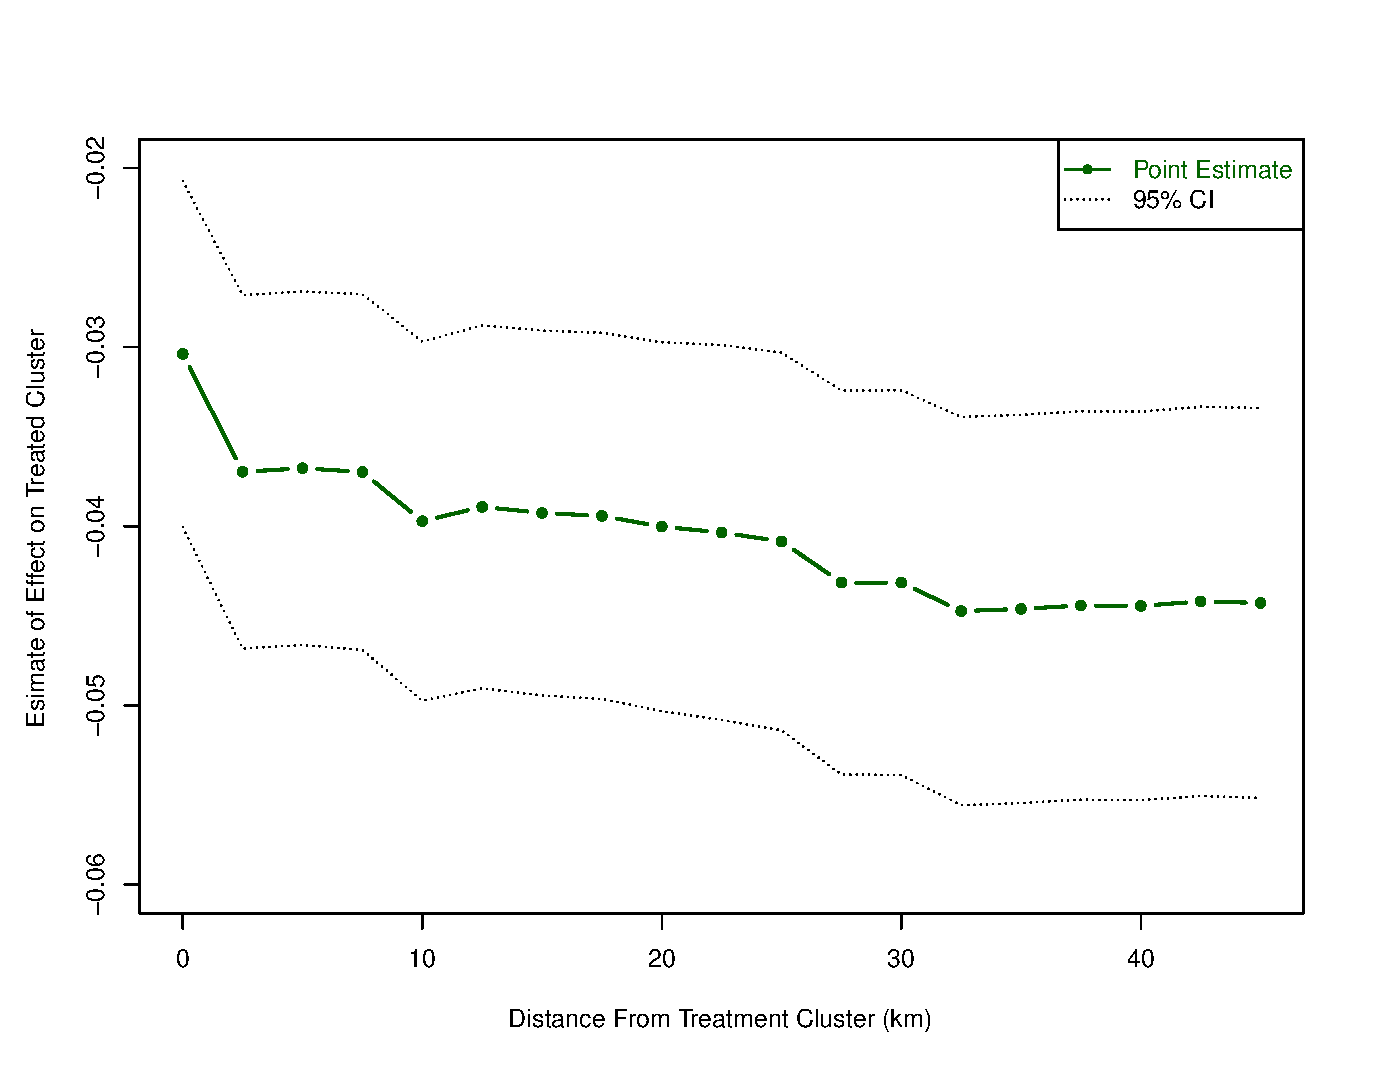
\includegraphics[scale=0.44]{./../../Figures/Dist2034.eps} 
\end{center}
\end{figure}
\hyperlink{dist1519}{\beamergotobutton{Back}}
\end{frame}


\begin{frame}
\begin{landscape}\begin{table}[htpb!]\centering
\caption{Emergency Contraception and Aggregate Human Capital} \label{TEENtab:PillAgg}
\begin{tabular}{@{\extracolsep{5pt}}lccccccccc} \\
[-1.8ex]\hline\hline \\[-1.8ex] &\multicolumn{3}{c}{15-19 year olds} &\multicolumn{3}{c}{20-34 year olds} &\multicolumn{3}{c}{35-49 year olds} \\
\cmidrule(r){2-4} \cmidrule(r){5-7} \cmidrule(r){8-10}
\textsc{Panel A:}&(1)&(2)&(3)&(4)&(5)&(6)&(7)&(8)&(9) \\
\textsc{Mother Characteristics} & Yrs Educ & Working & Married& Yrs Educ & Working & Married & Yrs Educ & Working & Married\\ \midrule
 & & & & & & & & & \\
Morning After Pill & 0.022 & -0.002 & 0.000& 0.001 & -0.004* & -0.003& 0.061** & -0.004 & -0.001 \\
& (0.021) & (0.002) & (0.001)& (0.014) & (0.002) & (0.005)& (0.028) & (0.005) & (0.007) \\
 & & & & & & & & & \\
Observations & 131,605 & 131,746 & 131,614& 896,230 & 897,363 & 896,318& 198,885 & 199,472 & 198,906\\
$ R^2 $ &  0.02 & 0.01 & 0.01& 0.14 & 0.04 & 0.17& 0.21 & 0.03 & 0.247 \\
 & & & & & & & & & \\
 & & & & & & & & & \\ \midrule
\textsc{Panel B:}&(1)&(2)&(3)&(4)&(5)&(6)&(7)&(8)&(9) \\
\textsc{Child Characteristics} & Weight & Gestation & Length& Weight & Gestation & Length & Weight & Gestation & Length\\ \midrule
 & & & & & & & & & \\
Morning After Pill & -1.377 & -0.020 & 0.039& -0.636 & -0.023*** & 0.02& -4.923 & -0.016 & 0.030 \\
& (5.944) & (0.019) & (0.028)& (2.532) & (0.008) & (0.016)& (5.602) & (0.016) & (0.024) \\
 & & & & & & & & & \\
Observations & 131,746 & 131,471 & 129,880& 897,363 & 895,671 & 885,932& 199,472 & 198,745 & 195,863\\
$ R^2 $ & 0.01 & 0.01 & 0.03& 0.01 & 0.01 & 0.03& 0.09 & 0.01 & 0.03 \\ \hline \hline \\[-1.8ex]
\multicolumn{10}{p{21cm}}{\begin{footnotesize}\textsc{Notes:} Each column represents an OLS regression, and full controls listed in table
\ref{TEENtab:PillPreg} are included.  Working and Married are binary variables, Weight is measured in grams, Gestation in weeks, and Length
in centimetres.  Summary statistics for these variables are available in table \ref{TEENtab:SumStats}.  Standard errors are clustered at the
 level of the municipality. $^{*}$ p $<0.1$; $^{**}$ p $<0.05$; $^{***}$ p $<0.01$.\end{footnotesize}}
\normalsize\end{tabular}\end{table}\end{landscape}

\end{frame}



\end{document}




%********************************************************************************
%********************************************************************************
%********************************************************************************
%********************************************************************************
%********************************************************************************
%********************************************************************************
%********************************************************************************
%********************************************************************************
%********************************************************************************
%********************************************************************************
